\documentclass[11pt, a4paper]{article}

% --- Geometry & Page Setup ---
\usepackage[a4paper, margin=2.5cm]{geometry}

% --- Font & Language Configuration ---
\usepackage[T1]{fontenc}
\usepackage[utf8]{inputenc}
\usepackage[english]{babel}
\usepackage{helvet}
\renewcommand{\familydefault}{\sfdefault}

% --- Essential Packages ---
\usepackage{amsmath, amssymb}
\usepackage{booktabs}
\usepackage{xcolor}
\usepackage{listings}
\usepackage{enumitem}
\usepackage{graphicx}
\usepackage{hyperref}

% --- Custom Color Definitions ---
\definecolor{brandblue}{RGB}{30, 58, 138}
\definecolor{brandaccent}{RGB}{13, 148, 136}
\definecolor{codebg}{RGB}{248, 250, 252}
\definecolor{codeframe}{RGB}{226, 232, 240}
\definecolor{commentgray}{RGB}{100, 116, 139}

% --- Setup Hyperlinks ---
\hypersetup{
    colorlinks=true,
    linkcolor=brandblue,
    citecolor=brandaccent,
    urlcolor=brandblue,
    pdftitle={Final Report - Advanced Control Systems},
    pdfauthor={Filippo Segalla}
}

% --- Setup Listings (Code Environment) ---
\lstset{
    backgroundcolor=\color{codebg},
    basicstyle=\ttfamily\scriptsize,
    breaklines=true,
    breakatwhitespace=false,
    captionpos=b,
    commentstyle=\color{commentgray},
    frame=single,
    rulecolor=\color{codeframe},
    keywordstyle=\color{brandblue}\bfseries,
    stringstyle=\color{brandaccent},
    showstringspaces=false,
    tabsize=2
}

% --- Custom Section Title Formatting ---
\makeatletter
\renewcommand{\section}{\@startsection{section}{1}{\z@}%
    {-3.5ex \@plus -1ex \@minus -.2ex}%
    {2.3ex \@plus .2ex}%
    {\normalfont\Large\bfseries\color{brandblue}}}
\renewcommand{\subsection}{\@startsection{subsection}{2}{\z@}%
    {-3.25ex \@plus -1ex \@minus -.2ex}%
    {1.5ex \@plus .2ex}%
    {\normalfont\large\bfseries\color{brandaccent}}}
\makeatother

% --- Document Metadata ---
\title{
    \vspace{-1cm}
    \color{brandblue}\textbf{Advanced Control Systems}\\[0.3em]
    \Large\textbf{Final Report: Collected Assignments}
}
\author{\textbf{Student Name:} Filippo Segalla \quad|\quad \textbf{Student ID:} VR538212\\[0.2em]
\small Department of Engineering for Innovative Medicine (DIMI) }
\date{\today}

\begin{document}

\maketitle
\thispagestyle{empty}

\tableofcontents
\newpage

% ==============================================================================
% ASSIGNMENT 1
% ==============================================================================
\section{Assignment 1}
\label{sec:assignment1}

\begin{abstract}
\noindent
This report presents a rigorous kinematic modeling and validation study for a 3-DOF PRR (Prismatic-Revolute-Revolute) robotic manipulator specified by a custom URDF description (\texttt{00001\_PRR\_zzx FILIPPO SEGALLA.urdf}). The report details the theoretical foundation, physical rationale, and mathematical derivation behind every stage of analysis: the Denavit-Hartenberg (D-H) frame alignment, direct kinematics transformations, analytical closed-form inverse kinematics, and the derivation of both Geometric ($\mathbf{J}_G$) and Analytical ($\mathbf{J}_a$) Jacobians. Each mathematical development is paired with an explanatory rationale answering \emph{what} operation is conducted and \emph{why} it is required in robot kinematics and control.
\end{abstract}

\hrule
\vspace{1.5em}

\subsection{System Architecture \& Kinematic Conventions}
\paragraph{What is being done:}
We model a 3-degree-of-freedom (3-DOF) spatial manipulator featuring a \textbf{PRR} architecture:
\begin{enumerate}[leftmargin=1.5em]
    \item \textbf{Joint 1 (Prismatic, $q_1$):} Translates vertically along the $Z_0$-axis, raising or lowering the entire arm structure.
    \item \textbf{Joint 2 (Revolute, $q_2$):} Rotates about a vertical axis parallel to $Z_0$, sweeping the arm across the horizontal plane.
    \item \textbf{Joint 3 (Revolute, $q_3$):} Rotates about a horizontal axis orthogonal to the second joint, providing elevation and reach in the vertical plane.
\end{enumerate}

\paragraph{Why it is done:}
Analyzing the kinematic structure before writing equations establishes the boundary conditions for the manipulator's workspace. Identifying joint types (prismatic vs. revolute) dictates the selection of columns in velocity Jacobians and determines whether joint displacement represents a spatial offset (meters) or a rotational angle (radians).

\begin{figure}[htbp]
    \centering
    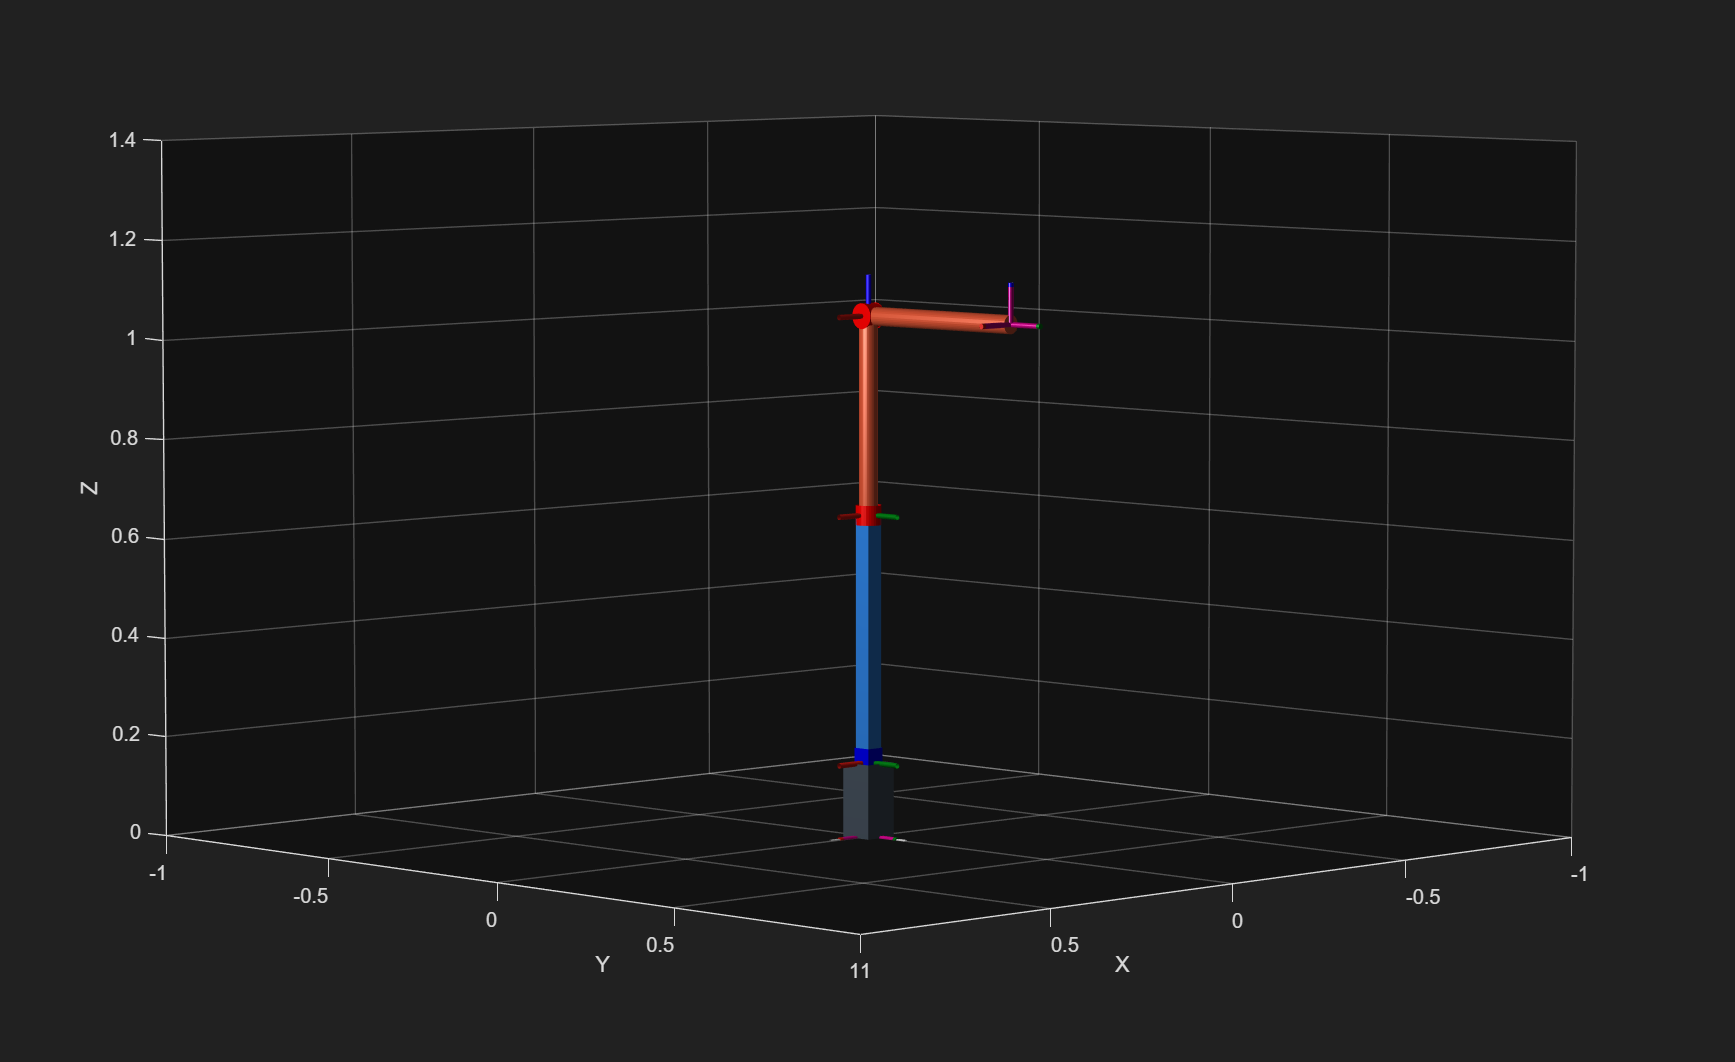
\includegraphics[width=0.8\textwidth, keepaspectratio]{../Images/RobotHomeConfiguration.png}
    \caption{PRR manipulator in its home configuration.}
    \label{fig:robot_home}
\end{figure}

\subsection{Joint Limits and Example Configurations}
\paragraph{What is being done:}
The movable-joint position limits are read from the robot URDF and checked before the kinematic calculations. The imported model specifies:
\begin{center}
\begin{tabular}{lcc}
\toprule
\textbf{Joint} & \textbf{Lower limit} & \textbf{Upper limit} \\
\midrule
$q_1$ (prismatic) & $-0.5\,\mathrm{m}$ & $0\,\mathrm{m}$ \\
$q_2$ (revolute) & $-\pi\,\mathrm{rad}$ & $\pi\,\mathrm{rad}$ \\
$q_3$ (revolute) & $-\pi\,\mathrm{rad}$ & $\pi\,\mathrm{rad}$ \\
\bottomrule
\end{tabular}
\end{center}
The MATLAB script prints these bounds and displays two admissible configurations:
\begin{itemize}[leftmargin=1.5em]
    \item $[-0.25,\,5\pi/6,\,\pi/3]$
    \item $[-0.40,\,\pi/4,\,-\pi/3]$
\end{itemize}
The coordinates are ordered as:
\begin{equation}
    [q_1,q_2,q_3]
\end{equation}

\begin{figure}[htbp]
    \centering
    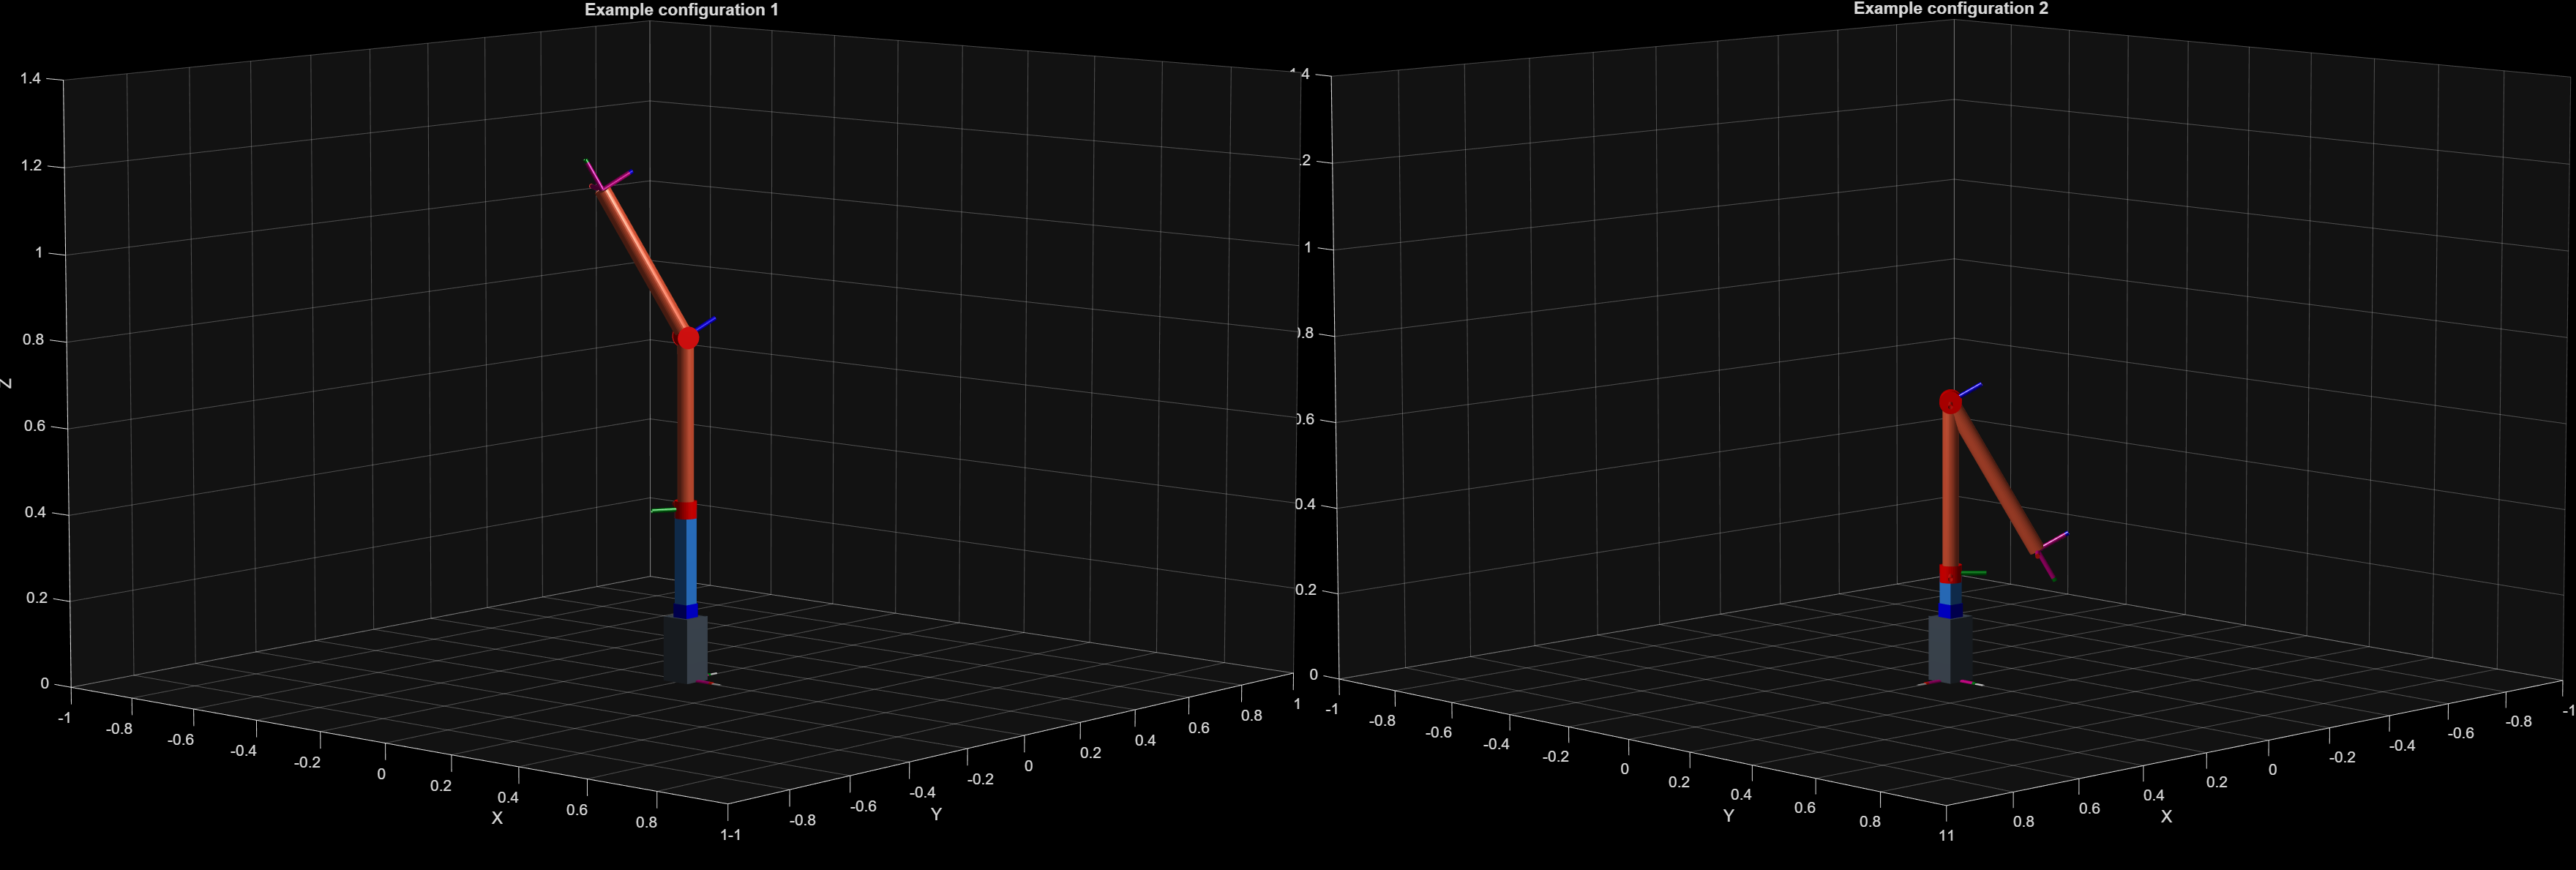
\includegraphics[width=\textwidth, keepaspectratio]{../Images/ExamplesConfiguration.png}
    \caption{The two admissible example configurations shown by the MATLAB script.}
    \label{fig:example_configurations}
\end{figure}

\paragraph{Why it is done:}
The URDF limits describe the robot's mechanically allowed range. Checking configurations against these limits prevents the visualization and inverse-kinematics output from presenting a mathematically valid pose that the physical manipulator cannot reach.

\subsection{Denavit-Hartenberg (D-H) Parameter Convention}
\paragraph{What is being done:}
We assign coordinate frames $F_0, F_1, F_2, F_3$ to each link following the standard Denavit-Hartenberg convention. The relative transformation between frame $i-1$ and frame $i$ is parameterized by four quantities: link length ($a_i$), link twist ($\alpha_i$), link offset ($d_i$), and joint angle ($\theta_i$).

The elementary transformation matrix $\mathbf{A}_i$ is constructed via four consecutive operations:
\begin{equation}
    \mathbf{A}_i = \text{Rot}_{z, \theta_i} \cdot \text{Trans}_{z, d_i} \cdot \text{Trans}_{x, a_i} \cdot \text{Rot}_{x, \alpha_i}
\end{equation}

Carrying out the matrix multiplication yields the explicit standard D-H matrix:
\begin{equation}
    \mathbf{A}_i = \begin{bmatrix}
    \cos\theta_i & -\sin\theta_i \cos\alpha_i & \sin\theta_i \sin\alpha_i & a_i \cos\theta_i \\
    \sin\theta_i & \cos\theta_i \cos\alpha_i & -\cos\theta_i \sin\alpha_i & a_i \sin\theta_i \\
    0 & \sin\alpha_i & \cos\alpha_i & d_i \\
    0 & 0 & 0 & 1
    \end{bmatrix}
\end{equation}

\paragraph{Why it is done:}
A general rigid-body transformation in 3D space requires 6 independent parameters (3 translational, 3 rotational). The D-H convention reduces this requirement to 4 parameters per link by enforcing strict geometric constraints (e.g., placing the $X_i$-axis along the common normal between $Z_{i-1}$ and $Z_i$). This systematic reduction simplifies symbolic computation, minimizes potential human error in matrix setup, and provides a unified standard across academic and industrial robotics frameworks.

\begin{table}[h!]
\centering
\caption{Denavit-Hartenberg parameters for the PRR Manipulator.}
\label{tab:dh_table}
\begin{tabular}{cccccc}
\toprule
\textbf{Link} $i$ & \textbf{Joint Type} & $a_i$ [m] & $\alpha_i$ [rad] & $d_i$ [m] & $\theta_i$ [rad] \\
\midrule
1 & Prismatic (P) & $0$ & $0$ & $q_1$ & $0$ \\
2 & Revolute (R)  & $0$ & $\pi/2$ & $0.4$ & $q_2$ \\
3 & Revolute (R)  & $0.4$ & $0$ & $0$ & $q_3$ \\
\bottomrule
\end{tabular}
\end{table}

\subsection{Direct Kinematics \& Frame Transformations}
\paragraph{What is being done:}
We incorporate two fixed transformation matrices, $\mathbf{T}_0^B$ and $\mathbf{T}_E^3$:
\begin{equation}
\mathbf{T}_0^B = \begin{bmatrix}
0 & -1 & 0 & 0 \\
1 & 0 & 0 & 0 \\
0 & 0 & 1 & 0.65 \\
0 & 0 & 0 & 1
\end{bmatrix}, \quad
\mathbf{T}_E^3 = \begin{bmatrix}
0 & 1 & 0 & 0 \\
0 & 0 & 1 & 0 \\
1 & 0 & 0 & 0 \\
0 & 0 & 0 & 1
\end{bmatrix}
\end{equation}

\paragraph{Why it is done:}
Standard D-H frames are placed based on geometric conveniences that rarely coincide with the actual physical world origin or the physical tool center point (TCP):
\begin{itemize}[leftmargin=1.5em]
    \item \textbf{Base Transformation ($\mathbf{T}_0^B$):} Relates the world coordinate system (e.g., ground level) to D-H Frame $0$. The vertical offset $0.65\text{ m}$ represents the fixed pedestal height of the robot base, while the $90^\circ$ $Z$-rotation aligns the internal D-H axis with the URDF coordinate system.
    \item \textbf{Tool Transformation ($\mathbf{T}_E^3$):} Re-aligns the axes of D-H Frame 3 with the actual end-effector flange orientation defined in the URDF, ensuring that position and orientation commands correspond to the true physical end-effector.
\end{itemize}

\subsection{Cumulative Kinematic Transformations}
\paragraph{What is being done:}
The cumulative transformation from the base frame to the $i$-th frame is computed by sequential matrix multiplication:
\begin{equation}
    \mathbf{T}_i^0(q) = \mathbf{T}_0^B \cdot \mathbf{A}_1(q_1) \cdots \mathbf{A}_i(q_i)
\end{equation}

Evaluating these multiplications symbolically yields:
\begin{equation}
\mathbf{T}_1^0(q) = \begin{bmatrix}
0 & -1 & 0 & 0 \\
1 & 0 & 0 & 0 \\
0 & 0 & 1 & q_1 + 0.65 \\
0 & 0 & 0 & 1
\end{bmatrix}
\end{equation}

\begin{equation}
\mathbf{T}_2^0(q) = \begin{bmatrix}
-\sin q_2 & 0 & \cos q_2 & 0 \\
\cos q_2 & 0 & \sin q_2 & 0 \\
0 & 1 & 0 & q_1 + 1.05 \\
0 & 0 & 0 & 1
\end{bmatrix}
\end{equation}

\begin{equation}
\mathbf{T}_3^0(q) = \begin{bmatrix}
-\sin q_2 \cos q_3 & \sin q_2 \sin q_3 & \cos q_2 & -0.4 \sin q_2 \cos q_3 \\
\cos q_2 \cos q_3 & -\sin q_3 \cos q_2 & \sin q_2 & 0.4 \cos q_2 \cos q_3 \\
\sin q_3 & \cos q_3 & 0 & q_1 + 0.4 \sin q_3 + 1.05 \\
0 & 0 & 0 & 1
\end{bmatrix}
\end{equation}

Multiplying $\mathbf{T}_3^0(q)$ by the end-effector transform $\mathbf{T}_E^3$ gives the final Direct Kinematics matrix $\mathbf{T}_E^B(q)$:
\begin{equation}
\mathbf{T}_E^B(q) = \begin{bmatrix}
\cos q_2 & -\sin q_2 \cos q_3 & \sin q_2 \sin q_3 & -0.4 \sin q_2 \cos q_3 \\
\sin q_2 & \cos q_2 \cos q_3 & -\sin q_3 \cos q_2 & 0.4 \cos q_2 \cos q_3 \\
0 & \sin q_3 & \cos q_3 & q_1 + 0.4 \sin q_3 + 1.05 \\
0 & 0 & 0 & 1
\end{bmatrix}
\end{equation}

Extracting the 4th column yields the operational position vector $\mathbf{p}_e = [p_x, p_y, p_z]^T$:
\begin{equation}
    \mathbf{p}_e(q) = \begin{bmatrix}
    p_x \\ p_y \\ p_z
    \end{bmatrix} = \begin{bmatrix}
    -0.4 \sin q_2 \cos q_3 \\
    0.4 \cos q_2 \cos q_3 \\
    q_1 + 0.4 \sin q_3 + 1.05
    \end{bmatrix}
\end{equation}

\paragraph{Why it is done:}
Direct Kinematics provides the fundamental mapping $\mathbf{p}_e = f(q)$ necessary for path planning, collision detection, and workspace visualization. Knowing the exact position of every intermediate joint frame ($\mathbf{T}_1^0, \mathbf{T}_2^0, \mathbf{T}_3^0$) is also required later to compute the partial Jacobians and link centers of mass for dynamic modeling.

\subsection{Closed-Form Inverse Kinematics}
\paragraph{What is being done:}
Inverse Kinematics solves for the joint variables $q = [q_1, q_2, q_3]^T$ given a target Cartesian coordinate $\mathbf{p}_e = [p_x, p_y, p_z]^T$. We derive an exact closed-form analytical solution.

\paragraph{Derivation Steps:}
\begin{enumerate}[leftmargin=1.5em]
    \item \textbf{Solving for $q_3$:} Summing the squares of $p_x$ and $p_y$:
    \begin{equation}
        p_x^2 + p_y^2 = (-0.4 \sin q_2 \cos q_3)^2 + (0.4 \cos q_2 \cos q_3)^2 = 0.16 \cos^2 q_3 (\sin^2 q_2 + \cos^2 q_2) = 0.16 \cos^2 q_3
    \end{equation}
    Taking the square root gives:
    \begin{equation}
        \cos q_3 = \frac{\sqrt{p_x^2 + p_y^2}}{0.4}
    \end{equation}
    The sine component is determined via the Pythagorean identity $\sin q_3 = \pm \sqrt{1 - \cos^2 q_3}$.

    \item \textbf{Solving for $q_2$:} Dividing $-p_x$ by $p_y$:
    \begin{equation}
        \frac{-p_x}{p_y} = \frac{0.4 \sin q_2 \cos q_3}{0.4 \cos q_2 \cos q_3} = \frac{\sin q_2}{\cos q_2} = \tan q_2 \implies q_2 = \text{atan2}(-p_x, p_y)
    \end{equation}

    \item \textbf{Solving for $q_1$:} Rearranging the expression for $p_z$:
    \begin{equation}
        p_z = q_1 + 0.4 \sin q_3 + 1.05 \implies q_1 = p_z - 1.05 - 0.4 \sin q_3
    \end{equation}
\end{enumerate}

\subsection{Physical Rationale of Multiple Solutions (Elbow-Up vs. Elbow-Down)}
\paragraph{What is being done:}
Due to the sign ambiguity in $\sin q_3 = \pm \sqrt{1 - \cos^2 q_3}$, two valid kinematic branches are calculated:
\begin{itemize}[leftmargin=1.5em]
    \item \textbf{Branch 1 (Elbow-Up, $\sin q_3 > 0$):}
    \begin{equation}
        q_3^{(1)} = \text{atan2}\left(+\sqrt{1 - \cos^2 q_3}, \cos q_3\right), \quad q_1^{(1)} = p_z - 1.05 - 0.4 \sin q_3^{(1)}
    \end{equation}
    \item \textbf{Branch 2 (Elbow-Down, $\sin q_3 < 0$):}
    \begin{equation}
        q_3^{(2)} = \text{atan2}\left(-\sqrt{1 - \cos^2 q_3}, \cos q_3\right), \quad q_1^{(2)} = p_z - 1.05 - 0.4 \sin q_3^{(2)}
    \end{equation}
\end{itemize}

\paragraph{Why it is done:}
Analytical closed-form solutions are computationally far superior to numerical iterative solvers (such as Newton-Raphson) because they compute in deterministic execution time ($O(1)$ complexity) and reveal all possible physical configurations. In real-time trajectory control, having access to both branches allows the controller to select the configuration that avoids mechanical joint limits, prevents self-collisions, or minimizes energy consumption.

\subsection{Filtering Solutions with the URDF Joint Limits}
Each analytical branch is evaluated numerically and compared component-wise with the limits in the URDF. A branch is accepted only if all three coordinates satisfy their respective lower and upper bounds; a branch outside any bound is reported and omitted from the robot visualization.

For the script's target $[p_x,p_y,p_z]=[0.25,0.25,0.9]\,\mathrm{m}$, both branches are mathematically feasible. They have approximately:
\begin{align*}
\text{Branch 1: } &[q_1,q_2,q_3] \approx [-0.3371,-0.7854,0.4864], &&\text{accepted},\\
\text{Branch 2: } &[q_1,q_2,q_3] \approx [0.0371,-0.7854,-0.4864], &&\text{rejected}.
\end{align*}
Branch 2 violates the prismatic upper limit $q_1\leq 0\,\mathrm{m}$, so it is not a physically admissible robot configuration even though it solves the inverse-kinematics equations.

\begin{figure}[htbp]
    \centering
    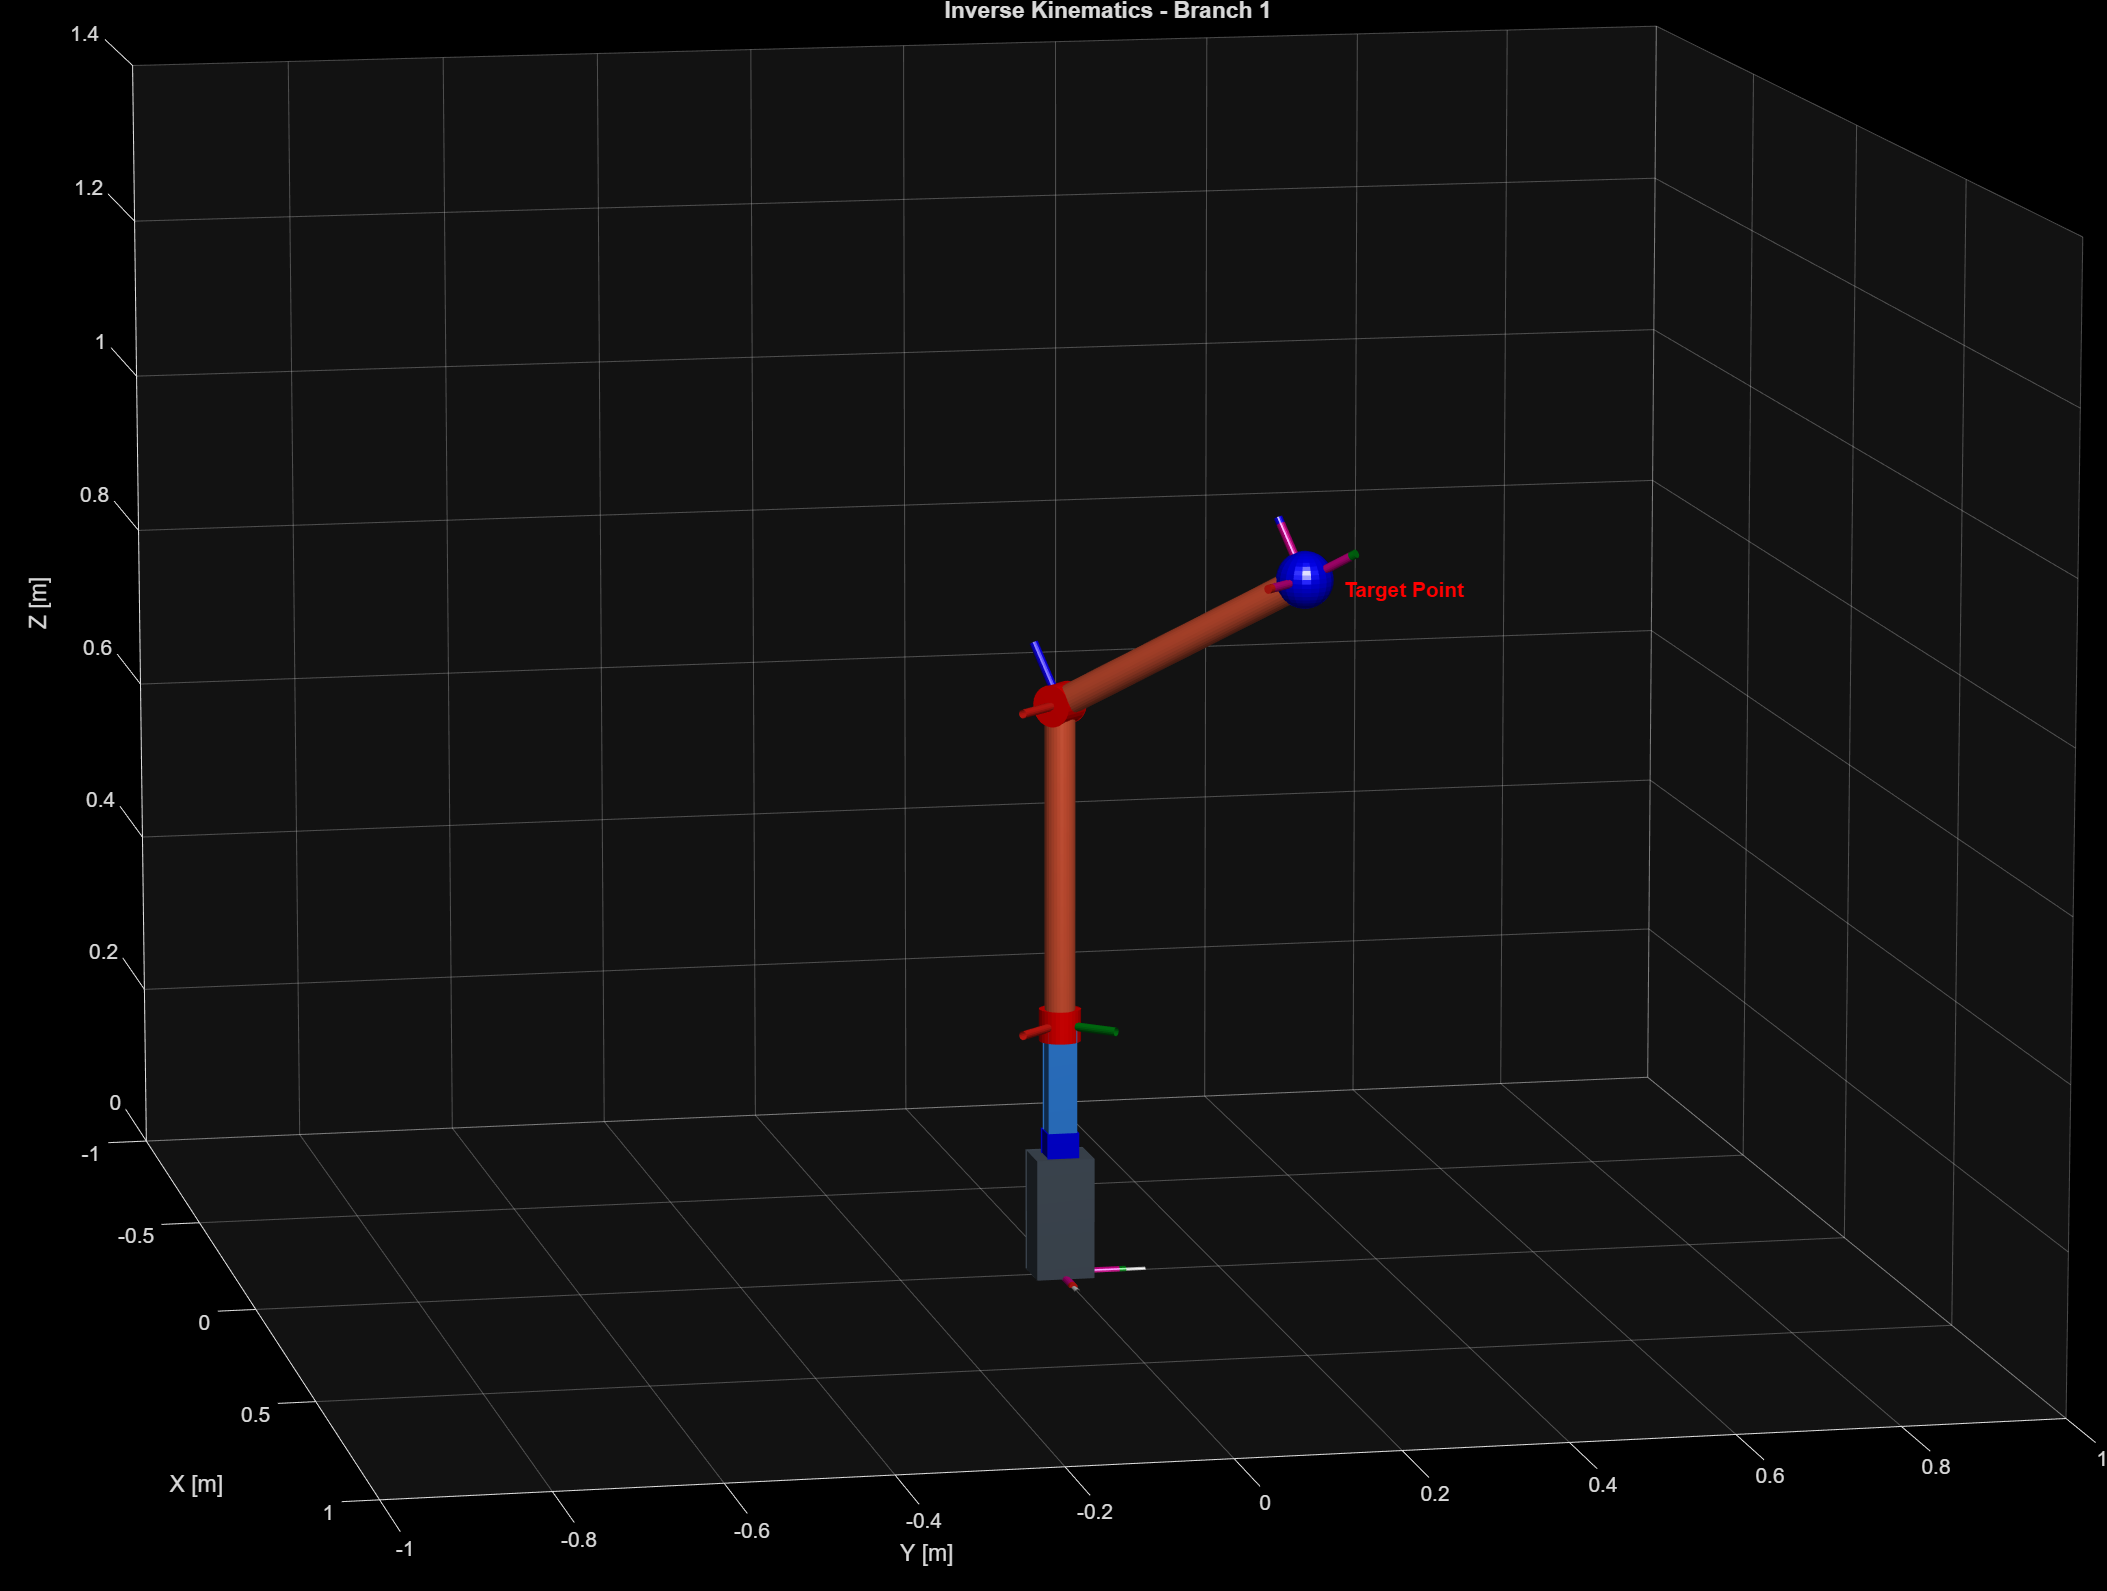
\includegraphics[width=\textwidth, keepaspectratio]{../Images/InverseKinematics.png}
    \caption{Inverse-kinematics visualization for the accepted elbow-up branch and target point.}
    \label{fig:inverse_kinematics}
\end{figure}

\subsection{\texorpdfstring{Geometric Jacobian ($\mathbf{J}_G$)}{Geometric Jacobian (JG)}}
\paragraph{What is being done:}
The Geometric Jacobian $\mathbf{J}_G(q) \in \mathbb{R}^{6 \times 3}$ relates joint velocities $\dot{q}$ directly to the linear ($\mathbf{v}_e$) and angular ($\boldsymbol{\omega}_e$) velocities of the end-effector in 3D physical space:
\begin{equation}
    \begin{bmatrix} \mathbf{v}_e \\ \boldsymbol{\omega}_e \end{bmatrix} = \mathbf{J}_G(q) \dot{q} = \begin{bmatrix} \mathbf{J}_{v1} & \mathbf{J}_{v2} & \mathbf{J}_{v3} \\ \mathbf{J}_{w1} & \mathbf{J}_{w2} & \mathbf{J}_{w3} \end{bmatrix} \begin{bmatrix} \dot{q}_1 \\ \dot{q}_2 \\ \dot{q}_3 \end{bmatrix}
\end{equation}

Columns are derived according to joint type:
\begin{itemize}[leftmargin=1.5em]
    \item \textbf{Prismatic Joint $i$:} $\mathbf{J}_{vi} = \mathbf{z}_{i-1}$, $\mathbf{J}_{wi} = \mathbf{0}$.
    \item \textbf{Revolute Joint $i$:} $\mathbf{J}_{vi} = \mathbf{z}_{i-1} \times (\mathbf{p}_e - \mathbf{p}_{i-1})$, $\mathbf{J}_{wi} = \mathbf{z}_{i-1}$.
\end{itemize}

\subsection{Column-by-Column Derivation}
\begin{enumerate}[leftmargin=1.5em]
    \item \textbf{Column 1 (Prismatic Joint 1):}
    $\mathbf{z}_0 = [0, 0, 1]^T \implies \mathbf{J}_{v1} = [0, 0, 1]^T, \quad \mathbf{J}_{w1} = [0, 0, 0]^T$.

    \item \textbf{Column 2 (Revolute Joint 2):}
    $\mathbf{z}_1 = [0, 0, 1]^T, \quad \mathbf{p}_1 = [0, 0, q_1 + 0.65]^T$.
    \begin{equation}
        \mathbf{J}_{v2} = \begin{bmatrix} 0 \\ 0 \\ 1 \end{bmatrix} \times \begin{bmatrix} -0.4 \sin q_2 \cos q_3 \\ 0.4 \cos q_2 \cos q_3 \\ 0.4 \sin q_3 + 0.4 \end{bmatrix} = \begin{bmatrix} -0.4 \cos q_2 \cos q_3 \\ -0.4 \sin q_2 \cos q_3 \\ 0 \end{bmatrix}, \quad \mathbf{J}_{w2} = \begin{bmatrix} 0 \\ 0 \\ 1 \end{bmatrix}
    \end{equation}

    \item \textbf{Column 3 (Revolute Joint 3):}
    $\mathbf{z}_2 = [\cos q_2, \sin q_2, 0]^T, \quad \mathbf{p}_2 = [0, 0, q_1 + 1.05]^T$.
    \begin{equation}
        \mathbf{J}_{v3} = \begin{bmatrix} \cos q_2 \\ \sin q_2 \\ 0 \end{bmatrix} \times \begin{bmatrix} -0.4 \sin q_2 \cos q_3 \\ 0.4 \cos q_2 \cos q_3 \\ 0.4 \sin q_3 \end{bmatrix} = \begin{bmatrix} 0.4 \sin q_2 \sin q_3 \\ -0.4 \sin q_3 \cos q_2 \\ 0.4 \cos q_3 \end{bmatrix}, \quad \mathbf{J}_{w3} = \begin{bmatrix} \cos q_2 \\ \sin q_2 \\ 0 \end{bmatrix}
    \end{equation}
\end{enumerate}

Assembling the complete $6 \times 3$ Geometric Jacobian:
\begin{equation}
\mathbf{J}_G(q) = \begin{bmatrix}
0 & -0.4 \cos q_2 \cos q_3 & 0.4 \sin q_2 \sin q_3 \\
0 & -0.4 \sin q_2 \cos q_3 & -0.4 \sin q_3 \cos q_2 \\
1 & 0 & 0.4 \cos q_3 \\
0 & 0 & \cos q_2 \\
0 & 0 & \sin q_2 \\
0 & 1 & 0
\end{bmatrix}
\end{equation}

\paragraph{Why it is done:}
The Geometric Jacobian is essential for:
\begin{enumerate}[leftmargin=1.5em]
    \item \textbf{Velocity Control:} Mapping desired Cartesian velocities to joint control commands
\begin{equation}
    \dot{q} = \mathbf{J}_G^\dagger \mathbf{v}
\end{equation}.
    \item \textbf{Singularity Analysis:} Singularity configurations occur when $\det(\mathbf{J}_G \mathbf{J}_G^T) = 0$ (e.g., when $\cos q_3 = 0$), where the robot loses a degree of freedom and required joint speeds approach infinity.
    \item \textbf{Statics \& Force Control:} Via the principle of virtual work, $\boldsymbol{\tau} = \mathbf{J}_G^T \mathbf{h}_e$, mapping end-effector contact forces $\mathbf{h}_e$ to joint torques $\boldsymbol{\tau}$.
\end{enumerate}

\subsection{\texorpdfstring{Analytical Jacobian ($\mathbf{J}_a$)}{Analytical Jacobian (Ja)}}
\paragraph{What is being done:}
The Analytical Jacobian $\mathbf{J}_a(q) \in \mathbb{R}^{6 \times 3}$ is obtained by directly differentiating the operational pose vector $\mathbf{x} = [\mathbf{p}_e^T, \boldsymbol{\phi}^T]^T$ with respect to joint coordinates $q$:
\begin{equation}
    \mathbf{J}_a(q) = \frac{\partial \mathbf{x}}{\partial q} = \begin{bmatrix} \frac{\partial \mathbf{p}_e}{\partial q} \\[0.4em] \frac{\partial \boldsymbol{\phi}}{\partial q} \end{bmatrix}
\end{equation}

Where $\boldsymbol{\phi} = [\phi, \theta, \psi]^T$ represents end-effector orientation parameterized by ZYZ Euler angles extracted from the rotation matrix $\mathbf{R}(q)$:
\begin{equation}
    \phi = q_2 + \frac{\pi}{2}, \quad \theta = q_3, \quad \psi = \frac{\pi}{2}
\end{equation}

Differentiating $\mathbf{p}_e$ and $\boldsymbol{\phi}$ yields:
\begin{equation}
\mathbf{J}_a(q) = \begin{bmatrix}
0 & -0.4 \cos q_2 \cos q_3 & 0.4 \sin q_2 \sin q_3 \\
0 & -0.4 \sin q_2 \cos q_3 & -0.4 \sin q_3 \cos q_2 \\
1 & 0 & 0.4 \cos q_3 \\
0 & 1 & 0 \\
0 & 0 & 1 \\
0 & 0 & 0
\end{bmatrix}
\end{equation}

\paragraph{Why it is done:}
Unlike angular velocity $\boldsymbol{\omega}_e$ (which is a vector quantity that cannot be directly integrated into a position coordinate), operational orientation angles $\boldsymbol{\phi}$ can be integrated. The Analytical Jacobian is therefore necessary for operational space control algorithms (e.g., Cartesian impedance control and PD pose tracking), where error feedback is expressed as a direct coordinate difference $\mathbf{e}_x = \mathbf{x}_d - \mathbf{x}$.

\newpage

% ==============================================================================
% ASSIGNMENT 2
% ==============================================================================
\section{Assignment 2}
\label{sec:assignment2}

\begin{abstract}
\noindent
This report presents the derivation of the total kinetic energy $\mathcal{T}(q, \dot{q})$, gravitational potential energy $\mathcal{U}(q)$, and generalized inertia matrix $\mathbf{B}(q)$ for a spatial 3-DOF PRR (Prismatic-Revolute-Revolute) robotic manipulator. Using König's theorem, partial Jacobians associated with link centers of mass (CoM), and local inertia tensors, closed-form parametric equations are established. The physical parameters are evaluated using exact rational symbolic arithmetic to prevent numerical round-off artifacts. Furthermore, numerical evaluation and 3D manipulator visualization are conducted at a sample configuration strictly respecting the URDF joint limits ($q_1 \in [-0.5, 0.0]\text{ m}$, $q_2, q_3 \in [-\pi, \pi]\text{ rad}$).
\end{abstract}

\hrule
\vspace{1.5em}

\subsection{System Architecture \& Mass Properties}
\paragraph{What is being done:}
The physical parameters extracted from the URDF file for each body link are defined as follows:
\begin{enumerate}[leftmargin=1.5em]
    \item \textbf{Link 1 (Prismatic Joint, $q_1$):} Mass $m_1 = 1.0\text{ kg}$, prismatic joint limit $q_1 \in [-0.5, 0.0]\text{ m}$. Geometry: rectangular bar ($0.036\text{ m} \times 0.036\text{ m} \times 0.5\text{ m}$).
    \item \textbf{Link 2 (Revolute Joint, $q_2$):} Mass $m_2 = 1.0\text{ kg}$, revolute joint limit $q_2 \in [-\pi, \pi]\text{ rad}$. Geometry: solid cylinder along $Z_2$ ($r = 0.019\text{ m}, h = 0.4\text{ m}$).
    \item \textbf{Link 3 (Revolute Joint, $q_3$):} Mass $m_3 = 1.0\text{ kg}$, revolute joint limit $q_3 \in [-\pi, \pi]\text{ rad}$. Geometry: solid cylinder along $X_3$ ($r = 0.019\text{ m}, h = 0.4\text{ m}$).
\end{enumerate}

\paragraph{Why it is done:}
Mass and inertia distribution dictate the dynamic response of the manipulator. Establishing accurate geometric inertia tensors relative to each link's Center of Mass (CoM) is required prior to applying Lagrangian energy principles.

\subsection{Energy Derivation via Lagrangian Mechanics}
\paragraph{What is being done:}
According to König's theorem, the total kinetic energy $\mathcal{T}(q, \dot{q})$ of an $n$-link manipulator is the sum of translational and rotational kinetic energies of all individual links:
\begin{equation}
    \mathcal{T}(q, \dot{q}) = \sum_{i=1}^{3} \left( \frac{1}{2} m_i \dot{\mathbf{p}}_{l_i}^T \dot{\mathbf{p}}_{l_i} + \frac{1}{2} \boldsymbol{\omega}_i^T \mathbf{I}_{l_i} \boldsymbol{\omega}_i \right) = \frac{1}{2} \dot{q}^T \mathbf{B}(q) \dot{q}
\end{equation}

Expressing CoM linear velocity $\dot{\mathbf{p}}_{l_i} = \mathbf{J}_{P}^{l_i}(q) \dot{q}$ and angular velocity $\boldsymbol{\omega}_i = \mathbf{J}_{O}^{l_i}(q) \dot{q}$ via partial Jacobians yields the generalized inertia matrix $\mathbf{B}(q)$:
\begin{equation}
    \mathbf{B}(q) = \sum_{i=1}^{3} \left( m_i (\mathbf{J}_{P}^{l_i})^T \mathbf{J}_{P}^{l_i} + (\mathbf{J}_{O}^{l_i})^T \mathbf{R}_i \mathbf{I}_{l_i}^i \mathbf{R}_i^T \mathbf{J}_{O}^{l_i} \right)
\end{equation}

\paragraph{Why it is done:}
The generalized inertia matrix $\mathbf{B}(q) \in \mathbb{R}^{3 \times 3}$ is symmetric and positive-definite ($\mathbf{B}(q) = \mathbf{B}(q)^T > 0$). It maps joint velocity vectors to generalized kinetic energy and constitutes the principal term in the manipulator dynamics.

\subsection{Potential Energy \texorpdfstring{$\mathcal{U}(q)$}{U(q)} Formulation}
\paragraph{What is being done:}
The gravitational potential energy $\mathcal{U}(q)$ is calculated as the sum of potential energies of the link centers of mass relative to the base frame $\Sigma_0$:
\begin{equation}
    \mathcal{U}(q) = -\sum_{i=1}^{3} m_i \mathbf{g}_0^T \mathbf{p}_{l_i}(q)
\end{equation}
where $\mathbf{g}_0 = [0, 0, -g]^T$ with $g = 9.81\text{ m/s}^2$.

Substituting the vertical CoM positions $z_{Ci}(q)$ yields:
\begin{equation}
    \mathcal{U}(q) = g \left[ m_1 (q_1 + 0.40) + m_2 (q_1 + 1.05) + m_3 \left( q_1 + 1.05 + 0.20 \sin q_3 \right) \right]
\end{equation}

Evaluating with link masses $m_i = 1\text{ kg}$:
\begin{equation}
    \mathcal{U}(q) = 9.81 \cdot \left[ 3 q_1 + 2.50 + 0.20 \sin q_3 \right] \text{ J}
\end{equation}

\paragraph{Why it is done:}
$\mathcal{U}(q)$ depends solely on joint position coordinates $q$. Its gradient:
\begin{equation}
    \mathbf{g}(q) = \nabla_q \mathcal{U}(q)
\end{equation}
represents the static joint torques required to compensate gravity.

\subsection{Closed-Form Inertia Matrix \texorpdfstring{$\mathbf{B}(q)$}{B(q)}}
Evaluating the symbolic terms yields:
\begin{equation}
\resizebox{\linewidth}{!}{$
\mathbf{B}(q) = \begin{bmatrix}
m_1 + m_2 + m_3 & 0 & \frac{m_3}{5}\cos q_3 \\[0.5em]
0 & I_{2yy} + I_{3yy}\cos^2 q_3 + I_{3xx}\sin^2 q_3 + \frac{m_3}{25}\cos^2 q_3 & 0 \\[0.5em]
\frac{m_3}{5}\cos q_3 & 0 & I_{3zz} + \frac{m_3}{25}
\end{bmatrix}
$}
\end{equation}

Substituting exact physical parameters yields the evaluated numerical matrix:
\begin{equation}
\mathbf{B}(q) = \begin{bmatrix}
3.0 & 0 & 0.2\cos q_3 \\
0 & 0.1068 - 0.05324\sin^2 q_3 & 0 \\
0.2\cos q_3 & 0 & 0.05342
\end{bmatrix}
\end{equation}

\subsection{Sample Numerical Evaluation \& 3D Visualization}
\paragraph{What is being done:}
To verify the physical validity of the energy model, we evaluate $\mathbf{B}(q)$, $\mathcal{T}(q, \dot{q})$, and $\mathcal{U}(q)$ at a specific configuration $q_{\text{sample}}$ strictly within URDF limits:
\begin{align}
    q_1 &= -0.25\text{ m} \quad (\text{URDF Limit: } [-0.5, 0.0]\text{ m}) \\
    q_2 &= \frac{\pi}{4}\text{ rad} \approx 0.7854\text{ rad} \quad (\text{URDF Limit: } [-\pi, \pi]\text{ rad}) \\
    q_3 &= \frac{\pi}{6}\text{ rad} \approx 0.5236\text{ rad} \quad (\text{URDF Limit: } [-\pi, \pi]\text{ rad})
\end{align}

Joint velocity vector: $\dot{q}_{\text{sample}} = [0.11\text{ m/s}, 0.13\text{ rad/s}, -0.27\text{ rad/s}]^T$.

\paragraph{Numerical Results:}
Evaluating at state $(q_{\text{sample}}, \dot{q}_{\text{sample}})$ yields:
\begin{equation}
\mathbf{B}(q_{\text{sample}}) = \begin{bmatrix}
3.0000 & 0 & 0.1732 \\
0 & 0.0535 & 0 \\
0.1732 & 0 & 0.0534
\end{bmatrix}
\end{equation}
\begin{align}
    \mathcal{T}(q_{\text{sample}}, \dot{q}_{\text{sample}}) &= 0.015406\text{ J} \\
    \mathcal{U}(q_{\text{sample}}) &= 18.148500\text{ J} \\
    \mathcal{E}_{\text{total}} = \mathcal{T} + \mathcal{U} &= 18.163906\text{ J}
\end{align}

\paragraph{Why it is done:}
This sample state provides concrete numerical validation of the mathematical energy equations and serves as a benchmark for controller verification.

\subsection{3D Robot Kinematic Visualization}
Figure \ref{fig:robot_visualization} shows the 3D plot of the 3-DOF PRR manipulator generated in MATLAB at the selected sample configuration $q_{\text{sample}} = [-0.25\text{ m}, 0.7854\text{ rad}, 0.5236\text{ rad}]^T$.

\begin{figure}[htbp]
    \centering
    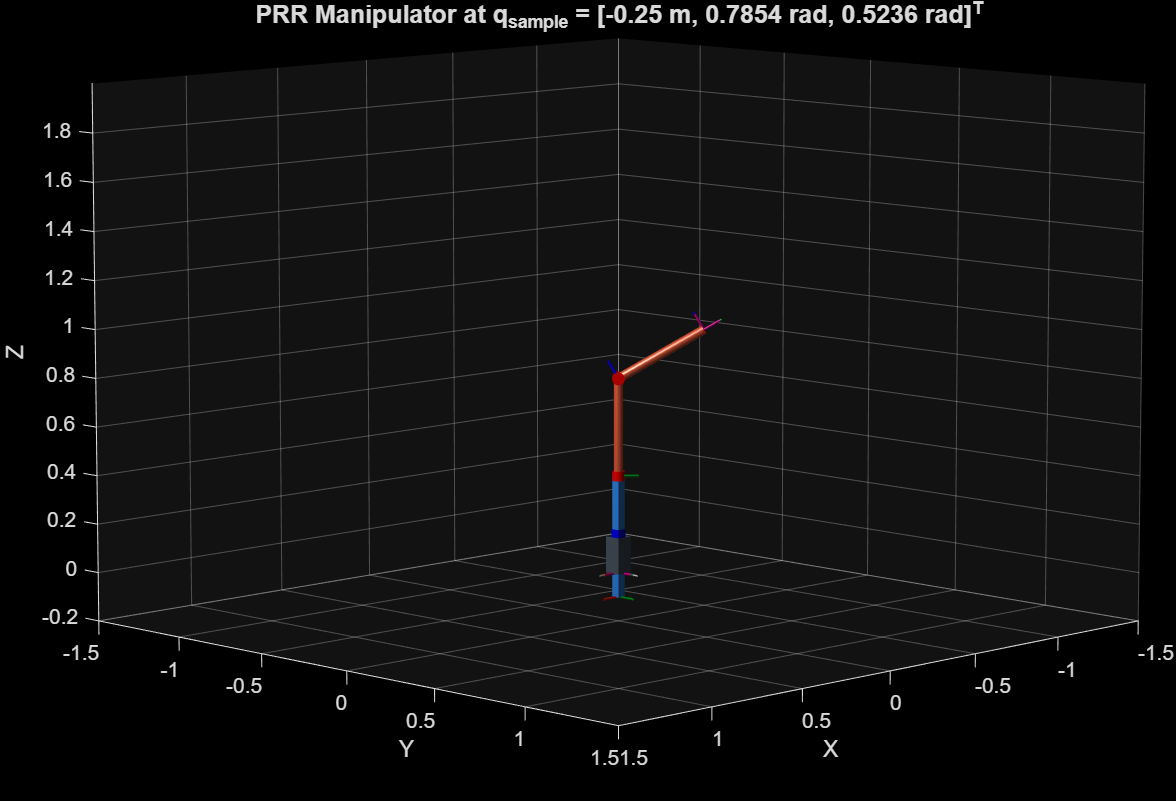
\includegraphics[width=0.85\linewidth]{../Images/KE_and_PE.png}
    \caption{3-DOF PRR Manipulator at $q_{\text{sample}} = [-0.25\text{ m}, 0.7854\text{ rad}, 0.5236\text{ rad}]^T$ strictly inside URDF joint limits.}
    \label{fig:robot_visualization}
\end{figure}

\newpage

% ==============================================================================
% ASSIGNMENT 3
% ==============================================================================
\section{Assignment 3}
\label{sec:assignment3}

\begin{abstract}
\noindent
This report presents the complete derivation and formal characterization of the dynamic equations of motion for a spatial 3-DOF PRR (Prismatic-Revolute-Revolute) robotic manipulator defined by the URDF specification (\texttt{00001\_PRR\_zzx} \texttt{FILIPPO} \texttt{SEGALLA.urdf}). Building upon the kinematic and dynamic energy results established in Assignment \#1 and Assignment \#2, the equations of motion are systematically derived in joint space using the Euler-Lagrange analytical mechanics framework: $\mathbf{B}(q)\ddot{q} + \mathbf{C}(q, \dot{q})\dot{q} + \mathbf{g}(q) = \boldsymbol{\tau}$. The Coriolis and centrifugal terms are computed component-by-component via Christoffel symbols of the first type. Furthermore, the essential structural passivity property—the skew-symmetry of the matrix $(\mathbf{\dot{B}}(q) - 2\mathbf{C}(q, \dot{q}))$—is analytically proven and numerically verified. Both parametric symbolic formulas and clean decimal numerical expressions evaluated with exact rational arithmetic are presented.
\end{abstract}

\hrule
\vspace{1.5em}

\subsection{System Architecture \& Dynamic Framework}
\paragraph{What is being done:}
We formulate the inverse dynamic model of the spatial 3-DOF PRR manipulator. The mechanical parameters extracted from the URDF file and validated in prior assignments are summarized as follows:
\begin{enumerate}[leftmargin=1.5em]
    \item \textbf{Link 1 (Prismatic Joint, $q_1$):} Mass $m_1 = 1.0\text{ kg}$, rectangular geometry ($0.036\text{ m} \times 0.036\text{ m} \times 0.5\text{ m}$).
    \item \textbf{Link 2 (Revolute Joint, $q_2$):} Mass $m_2 = 1.0\text{ kg}$, solid cylinder along $Z_2$ ($r = 0.019\text{ m}$, $h = 0.4\text{ m}$).
    \item \textbf{Link 3 (Revolute Joint, $q_3$):} Mass $m_3 = 1.0\text{ kg}$, solid cylinder along $X_3$ ($r = 0.019\text{ m}$, $h = 0.4\text{ m}$).
\end{enumerate}

\paragraph{Why it is done:}
Establishing the dynamic equations of motion is indispensable for model-based robot control, trajectory simulation, and joint actuator sizing. While kinematics maps motion geometry, dynamics couples joint forces and torques $\boldsymbol{\tau}$ to joint accelerations $\ddot{q}$, velocities $\dot{q}$, and positions $q$.

\subsection{Euler-Lagrange Analytical Method}
\paragraph{What is being done:}
The dynamics are derived using the scalar Lagrangian function \\$\mathcal{L}(q, \dot{q}) = \mathcal{T}(q, \dot{q}) - \mathcal{U}(q)$, defined as the difference between total kinetic energy $\mathcal{T}$ and total potential energy $\mathcal{U}$. The fundamental Euler-Lagrange equations of motion are given by:
\begin{equation}
    \frac{d}{dt}\left(\frac{\partial \mathcal{L}}{\partial \dot{q}_i}\right) - \frac{\partial \mathcal{L}}{\partial q_i} = \tau_i, \quad i = 1, 2, 3
\end{equation}

Substituting $\mathcal{L} = \frac{1}{2}\dot{q}^T \mathbf{B}(q)\dot{q} - \mathcal{U}(q)$ into the variational formulation yields the step-by-step derivatives:
\begin{align}
    \left(\frac{\partial \mathcal{L}}{\partial \dot{q}}\right)^T &= \mathbf{B}(q)\dot{q} \\
    \frac{d}{dt}\left(\frac{\partial \mathcal{L}}{\partial \dot{q}}\right)^T &= \mathbf{B}(q)\ddot{q} + \mathbf{\dot{B}}(q)\dot{q} \\
    \left(\frac{\partial \mathcal{L}}{\partial q}\right)^T &= \frac{1}{2}\left(\frac{\partial}{\partial q}\left(\dot{q}^T \mathbf{B}(q)\dot{q}\right)\right)^T - \left(\frac{\partial \mathcal{U}}{\partial q}\right)^T
\end{align}

Combining terms yields the canonical matrix differential equation:
\begin{equation}
    \mathbf{B}(q)\ddot{q} + \mathbf{C}(q, \dot{q})\dot{q} + \mathbf{g}(q) = \boldsymbol{\tau}
\end{equation}

\paragraph{Why it is done:}
The Euler-Lagrange method avoids computing internal constraint forces between links (unlike Newton-Euler vector mechanics) and directly delivers the generalized forces $\boldsymbol{\tau}$ performing work on the generalized coordinates $q$.

\subsection{Derivation of Dynamic Matrices}
\paragraph{What is being done:}
The symmetric, positive-definite inertia matrix $\mathbf{B}(q) \in \mathbb{R}^{3 \times 3}$ derived in Assignment \#2 is given symbolically by:
\begin{equation}
\resizebox{\linewidth}{!}{$
\mathbf{B}(q) = \begin{bmatrix}
m_1 + m_2 + m_3 & 0 & \frac{m_3}{5}\cos q_3 \\[0.5em]
0 & I_{2yy} + I_{3yy}\cos^2 q_3 + I_{3xx}\sin^2 q_3 + \frac{m_3}{25}\cos^2 q_3 & 0 \\[0.5em]
\frac{m_3}{5}\cos q_3 & 0 & I_{3zz} + \frac{m_3}{25}
\end{bmatrix}
$}
\end{equation}

Evaluated numerically:
\begin{equation}
\mathbf{B}(q) = \begin{bmatrix}
3.0 & 0 & 0.2\cos q_3 \\
0 & 0.1068 - 0.05324\sin^2 q_3 & 0 \\
0.2\cos q_3 & 0 & 0.05342
\end{bmatrix}
\end{equation}

\paragraph{Why it is done:}
$\mathbf{B}(q)$ captures the configuration-dependent mass and inertia properties. The diagonal element $b_{ii}(q)$ represents the effective moment of inertia at joint $i$ when all other joints are locked, while off-diagonal elements $b_{ij}(q)$ represent inertial acceleration coupling between joint $j$ and joint $i$.

\subsection{Coriolis and Centrifugal Matrix \texorpdfstring{$\mathbf{C}(q, \dot{q})$}{C(q, dq)} via Christoffel Symbols}
\paragraph{What is being done:}
To construct $\mathbf{C}(q, \dot{q})$, we compute Christoffel symbols of the first type $c_{ijk}(q)$, defined as:
\begin{equation}
    c_{ijk}(q) = \frac{1}{2} \left( \frac{\partial b_{ij}}{\partial q_k} + \frac{\partial b_{ik}}{\partial q_j} - \frac{\partial b_{jk}}{\partial q_i} \right)
\end{equation}

The individual entries $c_{ij}(q, \dot{q})$ of matrix $\mathbf{C}$ are computed via velocity contraction:
\begin{equation}
    c_{ij}(q, \dot{q}) = \sum_{k=1}^{3} c_{ijk}(q) \dot{q}_k
\end{equation}

Evaluating all $27$ Christoffel symbols yields the explicit symbolic matrix:
\begin{equation}
\resizebox{\linewidth}{!}{$
\mathbf{C}(q, \dot{q}) = \begin{bmatrix}
0 & 0 & -\frac{m_3}{5}\dot{q}_3\sin q_3 \\[0.5em]
0 & \frac{25(I_{3xx}-I_{3yy})-m_3}{50}\dot{q}_3\sin(2q_3) & \frac{25(I_{3xx}-I_{3yy})-m_3}{50}\dot{q}_2\sin(2q_3) \\[0.5em]
0 & \frac{-25(I_{3xx}-I_{3yy})+m_3}{50}\dot{q}_2\sin(2q_3) & 0
\end{bmatrix}
$}
\end{equation}

Evaluating numerically with exact rational substitution yields:
\begin{equation}
\mathbf{C}(q, \dot{q}) = \begin{bmatrix}
0 & 0 & -0.2\dot{q}_3\sin q_3 \\[0.3em]
0 & -0.02662\dot{q}_3\sin(2q_3) & -0.02662\dot{q}_2\sin(2q_3) \\[0.3em]
0 & 0.02662\dot{q}_2\sin(2q_3) & 0
\end{bmatrix}
\end{equation}

\paragraph{Why it is done \& Physical Interpretation:}
\begin{itemize}[leftmargin=1.5em]
    \item \textbf{Centrifugal Effects ($h_{ijj}\dot{q}_j^2$):} Terms proportional to $\dot{q}_j^2$ represent centrifugal forces acting on joint $i$ due to rotation of link $j$. Note $h_{iii} \equiv 0$ always.
    \item \textbf{Coriolis Effects ($h_{ijk}\dot{q}_j\dot{q}_k$):} Terms proportional to $\dot{q}_j\dot{q}_k$ ($j \neq k$) represent Coriolis forces arising from simultaneous motion along multiple moving axes.
    \item \textbf{Christoffel Symmetry:} $c_{ijk} = c_{ikj}$ guarantees consistency across velocity products.
\end{itemize}

\subsection{Gravity Torque Vector \texorpdfstring{$\mathbf{g}(q)$}{g(q)}}
\paragraph{What is being done:}
The gravity force vector $\mathbf{g}(q) \in \mathbb{R}^3$ is derived as the gradient of potential energy $\mathcal{U}(q)$:
\begin{equation}
    g_i(q) = \frac{\partial \mathcal{U}(q)}{\partial q_i} \implies \mathbf{g}(q) = \begin{bmatrix} g(m_1 + m_2 + m_3) \\[0.4em] 0 \\[0.4em] \frac{g m_3}{5}\cos q_3 \end{bmatrix}
\end{equation}

Substituting $g = 9.81\text{ m/s}^2$ and link masses $m_i = 1\text{ kg}$:
\begin{equation}
    \mathbf{g}(q) = \begin{bmatrix} 29.43 \\[0.3em] 0 \\[0.3em] 1.962\cos q_3 \end{bmatrix}
\end{equation}

\paragraph{Why it is done:}
The gravity vector specifies the static holding forces/torques required to maintain equilibrium ($\ddot{q}=\mathbf{0}, \dot{q}=\mathbf{0}$). Joint 2 requires zero gravity torque ($g_2 = 0$) because rotation about $Z_0$ occurs purely in a horizontal plane.

\subsection{Passivity \& Skew-Symmetry Analysis}
\paragraph{What is being done:}
We compute the time derivative of the generalized inertia matrix:
\begin{equation}
    \mathbf{\dot{B}}(q) = \sum_{k=1}^3 \frac{\partial \mathbf{B}}{\partial q_k} \dot{q}_k
\end{equation}
\begin{equation}
\mathbf{\dot{B}}(q) = \begin{bmatrix}
0 & 0 & -\frac{m_3}{5}\dot{q}_3\sin q_3 \\[0.4em]
0 & \frac{25(I_{3xx}-I_{3yy})-m_3}{25}\dot{q}_3\sin(2q_3) & 0 \\[0.4em]
-\frac{m_3}{5}\dot{q}_3\sin q_3 & 0 & 0
\end{bmatrix}
\end{equation}

We then evaluate the matrix $\mathbf{N}(q, \dot{q}) = \mathbf{\dot{B}}(q) - 2\mathbf{C}(q, \dot{q})$:
\begin{equation}
\resizebox{\linewidth}{!}{$
\mathbf{N}(q, \dot{q}) = \begin{bmatrix}
0 & 0 & \frac{m_3}{5}\dot{q}_3\sin q_3 \\[0.4em]
0 & 0 & \frac{-25(I_{3xx}-I_{3yy})+m_3}{25}\dot{q}_2\sin(2q_3) \\[0.4em]
-\frac{m_3}{5}\dot{q}_3\sin q_3 & \frac{25(I_{3xx}-I_{3yy})-m_3}{25}\dot{q}_2\sin(2q_3) & 0
\end{bmatrix}
$}
\end{equation}

Checking transpose equality confirms $\mathbf{N}^T = -\mathbf{N}$, meaning $\mathbf{N} + \mathbf{N}^T = \mathbf{0}_{3\times3}$.

\paragraph{Why it is done \& Control Implications:}
Skew-symmetry of $(\mathbf{\dot{B}} - 2\mathbf{C})$ implies that for any vector $\mathbf{x} \in \mathbb{R}^3$:
\begin{equation}
    \mathbf{x}^T \left( \mathbf{\dot{B}}(q) - 2\mathbf{C}(q, \dot{q}) \right) \mathbf{x} = 0
\end{equation}

This fundamental property reflects conservation of energy: internal Coriolis and centrifugal forces perform zero net work on the manipulator. It is heavily exploited in constructing Lyapunov candidates for adaptive control, computed-torque control, and passivity-based control.

\subsection{Explicit Dynamic Equations of Motion}
Combining all terms into scalar equations $\tau_i = \sum_{j=1}^3 b_{ij}\ddot{q}_j + \sum_{j=1}^3 c_{ij}\dot{q}_j + g_i$ gives:

\subsection{Scalar Dynamic Equations}
\begin{align}
    \tau_1 &= 3.0\,\ddot{q}_1 + 0.2\cos(q_3)\,\ddot{q}_3 - 0.2\sin(q_3)\,\dot{q}_3^2 + 29.43 \\
    \tau_2 &= \left(0.1068 - 0.05324\sin^2 q_3\right)\ddot{q}_2 - 0.05324\sin(2q_3)\,\dot{q}_2\dot{q}_3 \\
    \tau_3 &= 0.05342\,\ddot{q}_3 + 0.2\cos(q_3)\,\ddot{q}_1 + 0.02662\sin(2q_3)\,\dot{q}_2^2 + 1.962\cos(q_3)
\end{align}

\subsection{Extension to General Dynamic Model}
If joint viscous friction $F_v \dot{q}$, Coulomb friction $F_s \text{sgn}(\dot{q})$, or an external environment wrench $h_e$ are present, the general dynamic equation expands to:
\begin{equation}
    \mathbf{B}(q)\ddot{q} + \mathbf{C}(q, \dot{q})\dot{q} + F_v \dot{q} + F_s \text{sgn}(\dot{q}) + \mathbf{g}(q) = \boldsymbol{\tau} - \mathbf{J}^T(q) h_e
\end{equation}

\newpage

% ==============================================================================
% ASSIGNMENT 4
% ==============================================================================
\section{Assignment 4}
\label{sec:assignment4}

\begin{abstract}
\noindent
This report addresses the Recursive Newton-Euler (RNE) formulation, linearity in dynamic parameters, base parameter reduction, and Least-Squares (LS) parameter identification for a spatial 3-DOF PRR (Prismatic-Revolute-Revolute) robotic manipulator defined by URDF specification (\texttt{00001\_PRR\_zzx} \texttt{FILIPPO} \texttt{SEGALLA.urdf}). First, the $O(n)$ recursive Newton-Euler vector algorithm (comprising forward velocity/acceleration propagation and backward force/torque propagation) is formulated and numerically verified against the Euler-Lagrange equations from Assignment \#3. Second, the dynamic model is restructured into linear form $\boldsymbol{\tau} = \mathbf{Y}(q, \dot{q}, \ddot{q})\boldsymbol{\Theta}$. A linear dependence analysis reduces the initial parameter set to a minimal $5$-element base parameter vector $\bar{\boldsymbol{\Theta}}$ with minimal regressor matrix $\mathbf{X}(q, \dot{q}, \ddot{q})$. Finally, dynamic parameter identification is executed using a persistent excitation trajectory, yielding exact numerical identification ($\text{error} < 10^{-15}$) with a well-conditioned stacked regressor matrix.
\end{abstract}

\hrule
\vspace{1.5em}

\subsection{Recursive Newton-Euler (RNE) Formulation}
\paragraph{What is being done:}
We implement the Recursive Newton-Euler (RNE) algorithm to compute inverse dynamics $\boldsymbol{\tau} = \text{RNE}(q, \dot{q}, \ddot{q}, \mathbf{g}_0)$. The method operates in two recursive sweeps:
\begin{enumerate}[leftmargin=1.5em]
    \item \textbf{Forward Recursion ($i = 1 \to 3$):} Propagates angular velocities $\boldsymbol{\omega}_i^i$, angular accelerations $\dot{\boldsymbol{\omega}}_i^i$, linear origin accelerations $\dot{\mathbf{p}}_i^i$, and center-of-mass (CoM) accelerations $\dot{\mathbf{p}}_{C_i}^i$ from the base to the end-effector.
    \item \textbf{Backward Recursion ($i = 3 \to 1$):} Solves Newton translational balance:
\begin{equation}
    \mathbf{f}_i^i - \mathbf{R}_{i+1}^i \mathbf{f}_{i+1}^{i+1} = m_i \dot{\mathbf{p}}_{C_i}^i
\end{equation}
and Euler rotational balance ($\boldsymbol{\mu}_i^i$) from the end-effector back to the base, projecting forces and/or torques onto joint motion axes $\mathbf{z}_0$ to obtain generalized actuation torques $\tau_i$.
\end{enumerate}

\paragraph{Why it is done:}
While the Lagrangian approach delivers closed-form equations of motion ($\mathbf{B}\ddot{q} + \mathbf{C}\dot{q} + \mathbf{g} = \boldsymbol{\tau}$) with $O(n^4)$ symbolic complexity, Newton-Euler vector recursion achieves $O(n)$ computational efficiency, making it the preferred method for real-time model-based control and dynamic simulation.

\subsection{Forward \& Backward Vector Equations}
\paragraph{Forward Equations ($i = 1 \dots 3$):}
For revolute joints ($i = 2, 3$):
\begin{align}
    \boldsymbol{\omega}_i^i &= (\mathbf{R}_i^{i-1})^T (\boldsymbol{\omega}_{i-1}^{i-1} + \dot{q}_i \mathbf{z}_0) \\
    \dot{\boldsymbol{\omega}}_i^i &= (\mathbf{R}_i^{i-1})^T (\dot{\boldsymbol{\omega}}_{i-1}^{i-1} + \ddot{q}_i \mathbf{z}_0 + \dot{q}_i \boldsymbol{\omega}_{i-1}^{i-1} \times \mathbf{z}_0) \\
    \dot{\mathbf{p}}_i^i &= (\mathbf{R}_i^{i-1})^T \dot{\mathbf{p}}_{i-1}^{i-1} + \dot{\boldsymbol{\omega}}_i^i \times \mathbf{r}_{i-1,i}^i + \boldsymbol{\omega}_i^i \times (\boldsymbol{\omega}_i^i \times \mathbf{r}_{i-1,i}^i)
\end{align}

For prismatic joint ($i = 1$):
\begin{equation}
    \dot{\mathbf{p}}_1^1 = (\mathbf{R}_1^0)^T (\dot{\mathbf{p}}_0^0 - \mathbf{g}_0 + \ddot{q}_1 \mathbf{z}_0)
\end{equation}

Center-of-Mass (CoM) linear acceleration for all links:
\begin{equation}
    \dot{\mathbf{p}}_{C_i}^i = \dot{\mathbf{p}}_i^i + \dot{\boldsymbol{\omega}}_i^i \times \mathbf{r}_{i,C_i}^i + \boldsymbol{\omega}_i^i \times (\boldsymbol{\omega}_i^i \times \mathbf{r}_{i,C_i}^i)
\end{equation}

\paragraph{Backward Equations ($i = 3 \dots 1$):}
\begin{align}
    \mathbf{f}_i^i &= \mathbf{R}_{i+1}^i \mathbf{f}_{i+1}^{i+1} + m_i \dot{\mathbf{p}}_{C_i}^i \\
    \boldsymbol{\mu}_i^i &= -\mathbf{f}_i^i \times (\mathbf{r}_{i-1,i}^i + \mathbf{r}_{i,C_i}^i) + \mathbf{R}_{i+1}^i \boldsymbol{\mu}_{i+1}^{i+1} + \mathbf{R}_{i+1}^i \mathbf{f}_{i+1}^{i+1} \times \mathbf{r}_{i,C_i}^i + \mathbf{I}_i^i \dot{\boldsymbol{\omega}}_i^i + \boldsymbol{\omega}_i^i \times (\mathbf{I}_i^i \boldsymbol{\omega}_i^i)
\end{align}

Joint Torque Projection:
\begin{equation}
    \tau_i = \begin{cases} (\mathbf{f}_i^i)^T (\mathbf{R}_i^{i-1})^T \mathbf{z}_0 & \text{for Prismatic Joint (Joint 1)} \\ (\boldsymbol{\mu}_i^i)^T (\mathbf{R}_i^{i-1})^T \mathbf{z}_0 & \text{for Revolute Joints (Joints 2, 3)} \end{cases}
\end{equation}

\subsection{Linearity in Dynamic Parameters \& Base Parameters}
\paragraph{What is being done:}
The dynamic model is expressed in linear regressor form:
\begin{equation}
    \boldsymbol{\tau} = \mathbf{B}(q)\ddot{q} + \mathbf{C}(q, \dot{q})\dot{q} + \mathbf{g}(q) = \mathbf{Y}(q, \dot{q}, \ddot{q}) \boldsymbol{\Theta}
\end{equation}

Where $\boldsymbol{\Theta} \in \mathbb{R}^{30}$ contains 10 standard physical parameters per link ($m_i, m_i \mathbf{r}_{C_i}^i, \mathbf{I}_{i}^i$).

\paragraph{Why it is done:}
Linearity in dynamic parameters allows decoupling state kinematics ($q, \dot{q}, \ddot{q}$) into matrix $\mathbf{Y}$ while keeping unknown inertial parameters in vector $\boldsymbol{\Theta}$, making system identification solvable via linear least-squares.

\subsection{Base Parameter Reduction (\texorpdfstring{$\bar{\boldsymbol{\Theta}}$}{theta\_base})}
\paragraph{What is being done:}
Not all 30 parameters independently affect joint torques. By eliminating unobservable parameters (zero columns in $\mathbf{Y}$) and grouping linearly dependent columns, we extract the minimal set of 5 base parameters $\bar{\boldsymbol{\Theta}} \in \mathbb{R}^5$:
\begin{equation}
    \bar{\boldsymbol{\Theta}} = \begin{bmatrix}
    \bar{\theta}_1 \\[0.2em]
    \bar{\theta}_2 \\[0.2em]
    \bar{\theta}_3 \\[0.2em]
    \bar{\theta}_4 \\[0.2em]
    \bar{\theta}_5
    \end{bmatrix} = \begin{bmatrix}
    m_1 + m_2 + m_3 \\[0.2em]
    m_3 \\[0.2em]
    I_{2yy} + I_{3yy} \\[0.2em]
    I_{3xx} - I_{3yy} \\[0.2em]
    I_{3zz}
    \end{bmatrix} = \begin{bmatrix}
    3.000000 \text{ kg} \\[0.2em]
    1.000000 \text{ kg} \\[0.2em]
    0.026847 \text{ kg}\cdot\text{m}^2 \\[0.2em]
    -0.013243 \text{ kg}\cdot\text{m}^2 \\[0.2em]
    0.013424 \text{ kg}\cdot\text{m}^2
    \end{bmatrix}
\end{equation}

The corresponding minimal base regressor matrix $\mathbf{X}(q, \dot{q}, \ddot{q}) \in \mathbb{R}^{3 \times 5}$ is given by:
\begin{equation}
\resizebox{\linewidth}{!}{$
\mathbf{X}(q, \dot{q}, \ddot{q}) = \begin{bmatrix}
\ddot{q}_1 + g & 0.2\ddot{q}_3\cos q_3 - 0.2\dot{q}_3^2\sin q_3 & 0 & 0 & 0 \\[0.4em]
0 & \frac{\ddot{q}_2}{25}\cos^2 q_3 - \frac{\dot{q}_2\dot{q}_3}{25}\sin q_3 \cos q_3 & \ddot{q}_2 & \ddot{q}_2\sin^2 q_3 + \dot{q}_2\dot{q}_3\sin(2q_3) & 0 \\[0.4em]
0 & 0.2\ddot{q}_1\cos q_3 + \frac{\ddot{q}_3}{25} - \frac{\dot{q}_2^2}{50}\sin(2q_3) + 0.2g\cos q_3 & 0 & -\frac{\dot{q}_2^2}{2} \sin(2q_3) & \ddot{q}_3
\end{bmatrix}
$}
\end{equation}

\paragraph{Why it is done:}
Reducing to base parameters guarantees full column rank for the stacked regressor matrix during system identification, preventing numerical ill-conditioning and matrix singularity.

\subsection{Dynamic Parameter Identification via Least-Squares}
\paragraph{What is being done:}
We collect $N = 500$ time samples along a persistently exciting sinusoidal trajectory ($q_1(t) = 0.5\sin t, q_2(t) = \cos(1.5t), q_3(t) = 0.8\sin(2t)$). Stacking $3N$ torque equations yields the linear system $\mathbf{W} \bar{\boldsymbol{\Theta}} = \mathbf{T}$, where $\mathbf{W} \in \mathbb{R}^{1500 \times 5}$ and $\mathbf{T} \in \mathbb{R}^{1500}$. The optimal parameter estimates are solved via Moore-Penrose pseudo-inverse:
\begin{equation}
    \hat{\bar{\boldsymbol{\Theta}}}_{LS} = (\mathbf{W}^T \mathbf{W})^{-1} \mathbf{W}^T \mathbf{T}
\end{equation}

\paragraph{Why it is done:}
Least-Squares identification provides an optimal, noise-resilient estimate of the manipulator's base parameters required for adaptive and model-based feedback linearizing controllers.

\subsection{Identification Results \& Condition Number}
Table \ref{tab:identification_results} summarizes the numerical identification performance:

\begin{table}[h!]
\centering
\caption{Base Parameter Identification Results via Least-Squares.}
\label{tab:identification_results}
\setlength{\tabcolsep}{4pt}
\begin{tabular}{lcccc}
\toprule
\textbf{Base Parameter} & \textbf{Symbolic Definition} & \textbf{Ground Truth} & \textbf{Estimated ($\hat{\bar{\theta}}_{LS}$)} & \textbf{Absolute Error} \\
\midrule
$\bar{\theta}_1$ & $m_1 + m_2 + m_3$ & $3.000000$ & $3.000000$ & $< 10^{-15}$ \\
$\bar{\theta}_2$ & $m_3$ & $1.000000$ & $1.000000$ & $0.00$ \\
$\bar{\theta}_3$ & $I_{2yy} + I_{3yy}$ & $0.026847$ & $0.026847$ & $< 10^{-15}$ \\
$\bar{\theta}_4$ & $I_{3xx} - I_{3yy}$ & $-0.013243$ & $-0.013243$ & $< 10^{-15}$ \\
$\bar{\theta}_5$ & $I_{3zz}$ & $0.013424$ & $0.013424$ & $< 10^{-15}$ \\
\bottomrule
\end{tabular}
\end{table}

The stacked regressor matrix condition number is $\text{cond}(\mathbf{W}) = 11.50$, proving high numerical stability and excellent trajectory excitation.

\newpage
\section{Assignment 5}

\newpage
\section{Assignment 6}

\newpage
\section{Assignment 7}

\newpage
\section{Assignment 8}

\newpage
\section{Assignment 9}

\newpage
\section{Assignment 10}
\end{document}
